\documentclass[9pt, handout]{beamer}

%!TEX root = ../notas_de_clase.tex

%preamble

%language
\usepackage[spanish,es-nodecimaldot]{babel}
\usepackage[utf8]{inputenc}
\usepackage{apacite}
\usepackage[absolute,overlay]{textpos}

%packages
\usepackage[Algoritmo]{algorithm}
\usepackage{algorithmicx}
\usepackage[noend]{algpseudocode}
\usepackage{mathtools}
\setlength {\marginparwidth}{2cm}
\usepackage{todonotes}
\usepackage{amsbsy}
\usepackage{amssymb}
\usepackage{amsmath,bm}
\usepackage{dsfont}

\usepackage{xcolor}
\providecommand{\sred}[1]{\textcolor{red}{#1}}
\providecommand{\sblue}[1]{\textcolor{blue}{#1}}
\providecommand{\red}[1]{\textcolor{red}{\text{#1}}}
\providecommand{\blue}[1]{\textcolor{blue}{\text{#1}}}
\providecommand{\redb}[1]{\textcolor{red}{\textbf{#1}}}
\providecommand{\blueb}[1]{\textcolor{blue}{\textbf{#1}}}
\usepackage{graphicx}
\usepackage{fancybox}
\usepackage{booktabs}
\usepackage{caption}
\usepackage{float}
%\usepackage[longend,ruled,algochapter,linesnumbered,lined,boxed,commentsnumbered,spanish]{algorithm2e}
%\usepackage[algo2e]{algorithm2e}
\usepackage{amssymb}
\usepackage{amstext}
\usepackage{bm}
\usepackage{wrapfig}
\usepackage{subcaption} % para_unsupervised_chapter

%formatting

\usepackage[export]{adjustbox}

%caption para figuras
\captionsetup[figure]{width=.8\linewidth, font=small,labelfont={bf},name={Fig.},labelsep=period}
\captionsetup[table]{width=.8\linewidth,font=small,labelfont={bf},name={Tabla},labelsep=period}



\ifx\byn\undefined
    \definecolor{my_blue}{HTML}{C2D5FF}
    \definecolor{my_red}{HTML}{FFC2C2}
    \definecolor{my_yellow}{HTML}{FFFFE0}
\else
    \definecolor{my_blue}{HTML}{FFFFFF}
    \definecolor{my_red}{HTML}{FFFFFF}
    \definecolor{my_yellow}{HTML}{FFFFFF}
\fi


\usepackage[framemethod=TikZ]{mdframed}
\mdfdefinestyle{discusion}{%
    %linecolor=black,
    %outerlinewidth=0pt,
    roundcorner=0pt,
    innertopmargin=5pt,
    innerbottommargin=5pt,
    innerrightmargin=20pt,
    innerleftmargin=20pt,
    backgroundcolor=my_blue}

\colorlet{Green}{green!90}


\mdfdefinestyle{ejemplo}{%
    %linecolor=black,
    %outerlinewidth=0pt,
    roundcorner=0pt,
    innertopmargin=5pt,
    innerbottommargin=5pt,
    innerrightmargin=20pt,
    innerleftmargin=20pt,
    backgroundcolor=my_yellow}


\mdfdefinestyle{pendiente}{%
    style = discusion, 
    backgroundcolor=my_red}


\RequirePackage{url}



%definitions
\def\td{{\text d}}
\def\cN{{\mathcal N}}
\def\cX{{\mathcal X}} 
\def\cC{{\mathcal C}} 
\def\N{{\mathbb N}}
\def\d{{\text d}}
\def\datos{{\mathcal D}}
\def\eye{{\mathbb I}}
\def\ssum{{\scriptstyle\sum}}
\def\bepsilon{{\bm \epsilon}}
\def\tx{\tilde{x}}
\def\tX{\tilde{X}}
\def\thetaMAP{\theta_\text{MAP}}
\newcommand{\gp}{\ensuremath{\mathcal{GP}}}
\newcommand{\pr}{\ensuremath{\mathbb{P}}}
\newcommand{\x}{\ensuremath{\mathbf{x}}}
\newcommand{\z}{\ensuremath{\mathbf{z}}}
\newcommand{\cvector}{\ensuremath{\mathbf{c}}}
\newcommand{\e}{\ensuremath{\mathbf{e}}}
\newcommand{\y}{\ensuremath{\mathbf{y}}}
\newcommand{\bx}{\ensuremath{\textcolor{blue}{X}}}
\newcommand{\by}{\ensuremath{\textcolor{blue}{Y}}}
\newcommand{\rx}{\ensuremath{\textcolor{red}{X_*}}}

\newcommand{\R}{\mathbb{R}}
\newcommand{\norm}[1]{\left\lVert#1\right\rVert}




\DeclareMathOperator*{\argmax}{arg\,max}
\DeclareMathOperator*{\argmin}{arg\,min}
\DeclareMathOperator{\E}{\mathbb{E}}
\DeclareMathOperator{\V}{\mathbb{V}}
\DeclareMathOperator{\KL}{\text{KL}}
\DeclareMathOperator{\MVN}{\text{MVN}}
\newcommand\deq{\stackrel{\mathclap{\normalfont\mbox{\tiny def}}}{=}}
%\newcommand{\E}[1]{\mathbb E \left[#1\right]}
\newcommand{\trace}[1]{\text{Tr} \left[#1\right]}


\usepackage{amsthm}

%-------------------------------------------
% Newtheorem
%-------------------------------------------
\newtheorem{axioma}{\textcolor{red}{Axioma}}
\newtheorem{definicion}{Definición}
\newtheorem*{notacion}{Notación}
\newtheorem{teorema}{Teorema}
\newtheorem{corolario}{Corolario}
\newtheorem{lema}{Lema}
\newtheorem{lemaZ}{\textcolor{red}{Lema}}
\newtheorem{propiedad}{Propiedad:}
\newtheorem{proposicion}{Proposición:}
\newtheorem*{observacion}{Observación}
\newtheorem*{comentario}{Comentario}
\newtheorem*{ejemplo}{Ejemplo}
\newtheorem*{resultado}{Resultado}
\newtheorem*{propuesto}{Ejercicio propuesto}
\newtheorem*{demostracion}{Demostración} % No se usa, usar \begin{proof}\end{proof} que son por default.

%listing paackage para código
\usepackage{listings}
\usepackage{xcolor}
 
\definecolor{codegreen}{rgb}{0,0.6,0}
\definecolor{codegray}{rgb}{0.5,0.5,0.5}
\definecolor{codepurple}{rgb}{0.58,0,0.82}
\definecolor{backcolour}{rgb}{0.95,0.95,0.92}
 
\lstdefinestyle{mystyle}{
    xleftmargin=0.15\textwidth,
    linewidth=0.8\textwidth,
    backgroundcolor=\color{backcolour},   
    commentstyle=\color{codegreen},
    keywordstyle=\color{magenta},
    numberstyle=\tiny\color{codegray},
    stringstyle=\color{codepurple},
    basicstyle=\ttfamily\footnotesize,
    breakatwhitespace=true,         
    breaklines=true,                 
    captionpos=b,                    
    keepspaces=true,                 
    numbers=left,                    
    numbersep=5pt,                  
    showspaces=false,                
    showstringspaces=false,
    showtabs=false,                  
    tabsize=2
}
 
\lstset{style=mystyle}

\numberwithin{equation}{section}

\usetheme{simple}

\title{Clase 15: Reducción de dimensionalidad}
\subtitle{MA5204 Aprendizaje de Máquinas}
\date{\today}
\author{Felipe Tobar} 
\titlegraphic{
\begin{figure}[htp] 
    \centering
        
\includegraphics[width=0.15\textwidth]{../img/Uchile.pdf}% 
\end{figure}
}
\institute{Department of Mathematical Engineering \&\\ Center for Mathematical Modelling\\Universidad de Chile}

\begin{document}
\begin{frame}
  \titlepage
\end{frame}

%Reducción de dimensionalidad.
\begin{frame}{Reducción de dimensionalidad}

El problema de reducción de dimensionalidad es parte del \textbf{aprendizaje no-supervisado} y consiste con construir una representación de dimensión estrictamente menor que los datos originales con la finalidad de interpretar de mejor forma la información contenida en nuestros datos así como también disminuir el costo computacional en el entrenamiento.\\~\ \pause

Hoy veremos dos técnicas de reducción de dimensionalidad:

\begin{itemize}
	\item Análisis de componentes principales (PCA).
	\item Discriminante lineal de Fisher.
\end{itemize}
	
\end{frame}

%Análisis de componentes principales (PCA): idea general.
\begin{frame}{Análisis de componentes principales (PCA): idea general}

Consideremos un conjunto de observaciones de $\{\x_i\}_{i=1}^N\subset\R^M$, se denotará por $x_{ij}$ al valor del atributo $j$ para la observación $i$. \\~\ \pause

Cada observación puede descomponerse en la base canónica $\{\e_i\}_{i=1}^M$ de $\R^M$ de la forma 
\begin{equation*}
	\x_i = x_{i1}\e_1 +  x_{i2}\e_2 + \cdots + x_{iM}\e_M.	
\end{equation*}\pause

Notemos que es posible aproximar cada observación $\x_i$ mediante una cantidad $M'<M$ de términos, truncando la representación anterior, es decir,  
\begin{equation*}
	\x_i \approx \sum_{j=1}^{M'} x_{i\sigma(j)}\e_{\sigma(j)}.
\end{equation*}

donde $\sigma:\{1,2,\ldots,M\}\mapsto\{1,2,\ldots,M\}$ es una permutación que prioriza las coordenadas más representativas de los datos. Dichas aproximaciones son una versión de baja dimensión de las observaciones $\{\x_i\}_{i=1}^N$.\\~\ 

$\star$ ¿qué es \textbf{más} representativa?
\end{frame}

%Análisis de componentes principales (PCA): criterio.
\begin{frame}{Análisis de componentes principales (PCA): criterio}
	
	Dada una dimensión $M'<M$:    	
	\begin{itemize}
		\item ¿es efectivamente un subconjunto de los vectores canónicos la mejor base para descomponer las observaciones? \pause
		\begin{figure}[H]
	\centering
	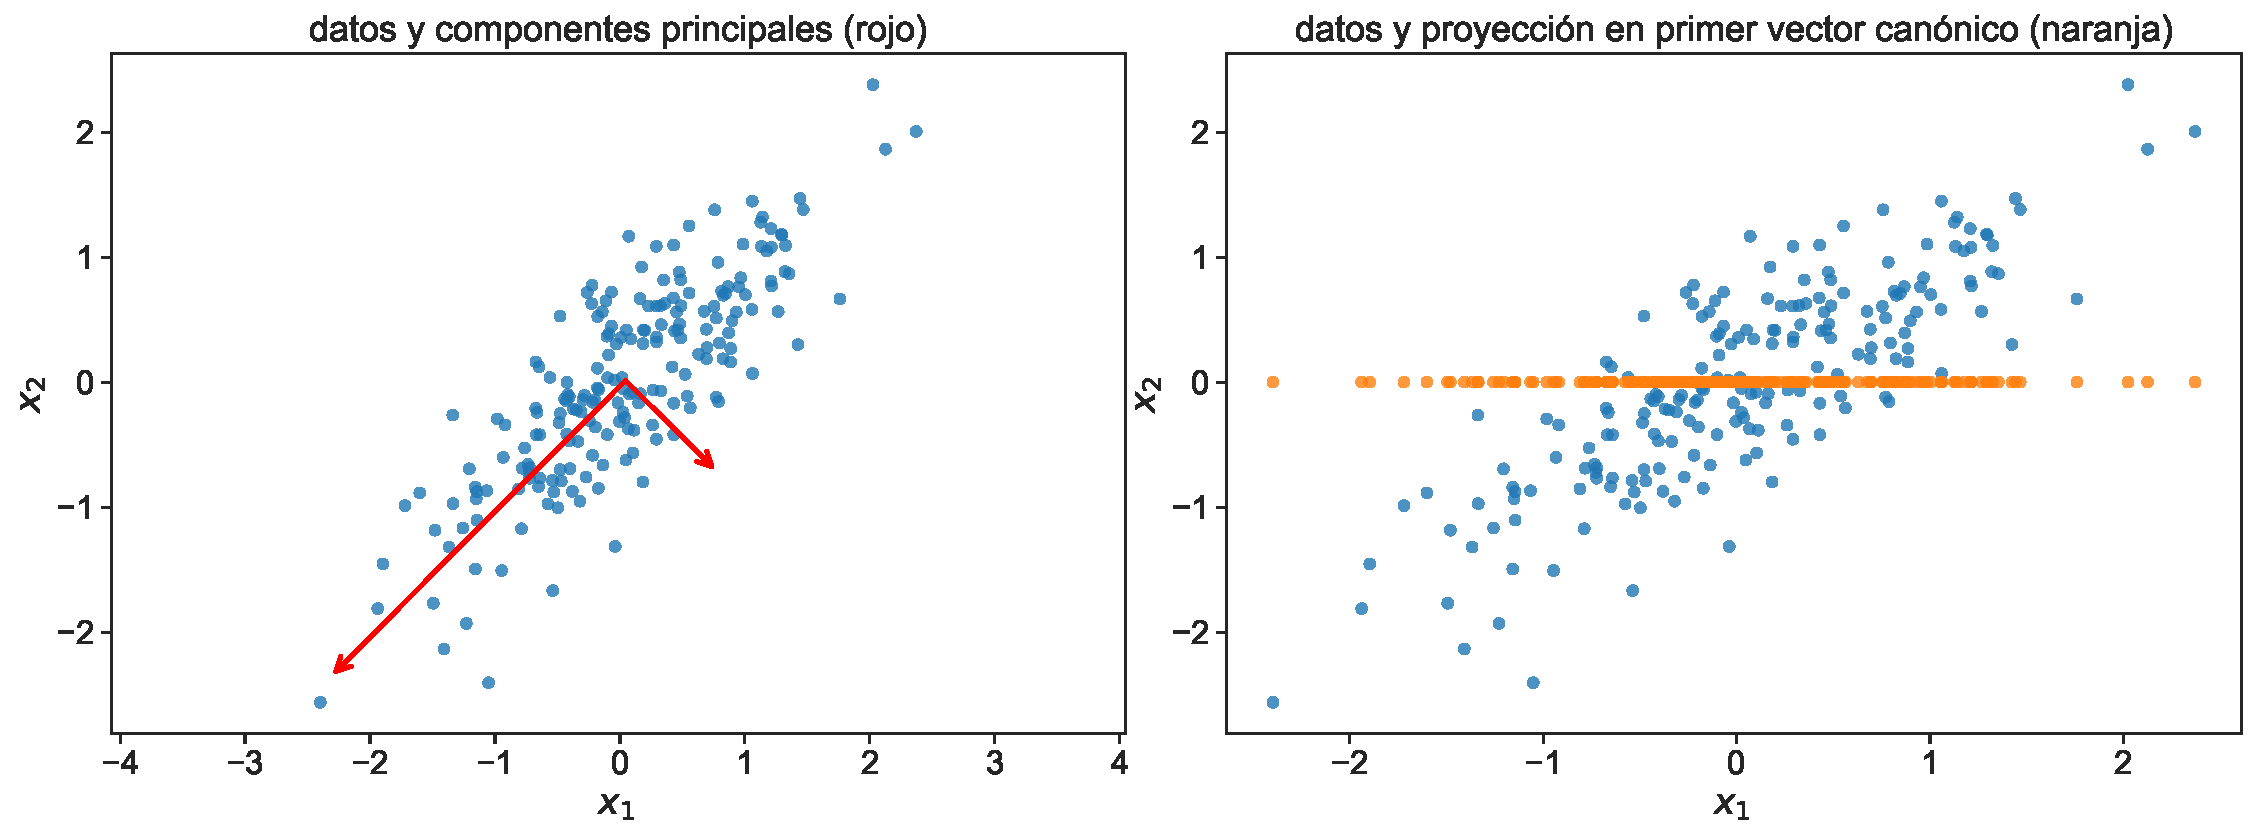
\includegraphics[width=0.6\textwidth]{../img/cap6_pca.pdf}
	\end{figure}\pause

		\item ¿cómo encontramos la \emph{mejor} base?\\~\ \pause
		
		Lo primero que se requiere es definir qué se entiende por \emph{mejor}. Nos enfocaremos en determinar una base cuyos componentes \textbf{ordenados} $\cvector_1,\cvector_2,\ldots$ capturan las $M'$ direcciones ortogonales de máxima variabilidad de nuestros datos.
	\end{itemize}
	Este criterio es conocido como \textbf{análisis de componentes principales (PCA)}.
\end{frame}


%Análisis de componentes principales (PCA): criterio.
\begin{frame}{Análisis de componentes principales (PCA): criterio}

De esta forma, dado que $\langle\cvector,\x\rangle$ representa la proyección ortogonal de $\x$ sobre $\cvector$, el primer elemento de la nueva base estará dado por 
\begin{equation*}
	\cvector_1 = \argmax_{||\cvector||=1} {\langle\cvector,\x\rangle}. \label{eq:PCA_max}
\end{equation*} \pause

\begin{itemize}
	\item La restricción $||\cvector_1||=1$ es necesaria ya que $\langle\lambda\cvector_1,\x\rangle = \lambda\langle\cvector_1,\x\rangle$ por lo que $\langle\cvector_1,\x\rangle$ puede crecer indefinidamente si no se fija una restricción sobre la norma de $\cvector$. \pause
	\item Además, es importante estandarizar los datos:\\~\ \pause

	\begin{enumerate}
	\item \textbf{Características de media nula:} la matriz $X$ debe tener columnas con media $0$. El objetivo de este ajuste es poder centrar los datos.\\~\ \pause
	\item \textbf{Varianzas marginales unitarias:} si una dimensión tiene una varianza marginal mayor que el resto, esta será más importante en la determinación de la dirección de máxima varianza solo por su magnitud y no por la relación entre variables.
	\end{enumerate}
\end{itemize}

	
\end{frame}

%Análisis de componentes principales (PCA): formulación.
\begin{frame}{PCA: Formulación}
En general no contamos con la distribución de las observaciones $p(\x)$, por lo que se puede considerar una aproximación muestral de la varianza y resolver 
\begin{align*}
	\cvector_1 = \argmax_{||\cvector||=1} \sum_{i=1}^N \langle\cvector,\x_i\rangle^2.\label{eq:PCA_max2}
\end{align*} \pause
Usando la siguiente notación
$$
X=\begin{bmatrix}
        \x_1^\top\\
        \vdots\\
        \x_N^\top\\
        \end{bmatrix}=
        \begin{bmatrix}
        {x}_{11}    & \dots & {x}_{1M}  \\
        \vdots          & \ddots& \vdots        \\
        {x}_{N1}    & \dots & {x}_{NM}
        \end{bmatrix},
$$
\pause
se puede reescribir el problema como
\begin{equation*}
	\cvector_1 = \argmax_{||\cvector||=1} ||X\cvector||^2 
			= \argmax_{||\cvector||=1} \cvector^\top X^\top X \cvector
			= \argmax_{\cvector} \frac{\cvector^\top X^\top X \cvector}{\cvector^\top \cvector}.
			\label{eq:PCA_max3}
\end{equation*}

\end{frame}


%Análisis de componentes principales (PCA): cociente de Rayleigh.
\begin{frame}{PCA: Cociente de Rayleigh}
	
Para el problema anterior, se tiene la siguiente propiedad:

\begin{lemma}[minimización del cociente de Rayleigh]

Sea $M\in\mathcal{M}_{nn}(\R)$ matriz cuadrada simétrica, entonces, para el cociente de Rayleigh

\begin{equation*}
	R(M,x):=\frac{x^\top Mx}{x^\top x},
\end{equation*}
se tiene que su valor mínimo corresponde al menor valor propio de $M$, y es alcanzado en su vector propio asociado.

\end{lemma}
\pause
De esta forma, dado que $X^\top X$ es simétrica, su cociente de Rayleigh es maximizado en el vector propio asociado al valor propio máximo de $X^\top X$.\\~\ \pause

Consecuentemente, la proyección de una observación $\x_i$ en la dirección de máxima varianza, o bien la \emph{primera componente principal}, está dada por 
\begin{equation*}
	\x_i^{(1)} = \langle \x_i, \cvector_1 \rangle,
\end{equation*}
donde $\cvector_1$ es el vector propio asociado al mayor valor propio de la matriz de covarianza muestral $XX^\top$.\\	
\end{frame}

%Kernel PCA.
\begin{frame}{Estudio personal: Kernel PCA}

Es posible utilizar el truco del kernel en PCA. En ese sentido, en vez de calcular la matriz de covarianza empírica $X^\top X$, se utiliza la matriz de Gram dada por un kernel $K$ donde

$$
K_{ij} = K(x_i,x_j) = \langle\phi(x_i),\phi(x_j)\rangle
$$

Luego, se realiza PCA utilizando dicha matriz.\\ \pause

\begin{figure}[ht]
    \centering
    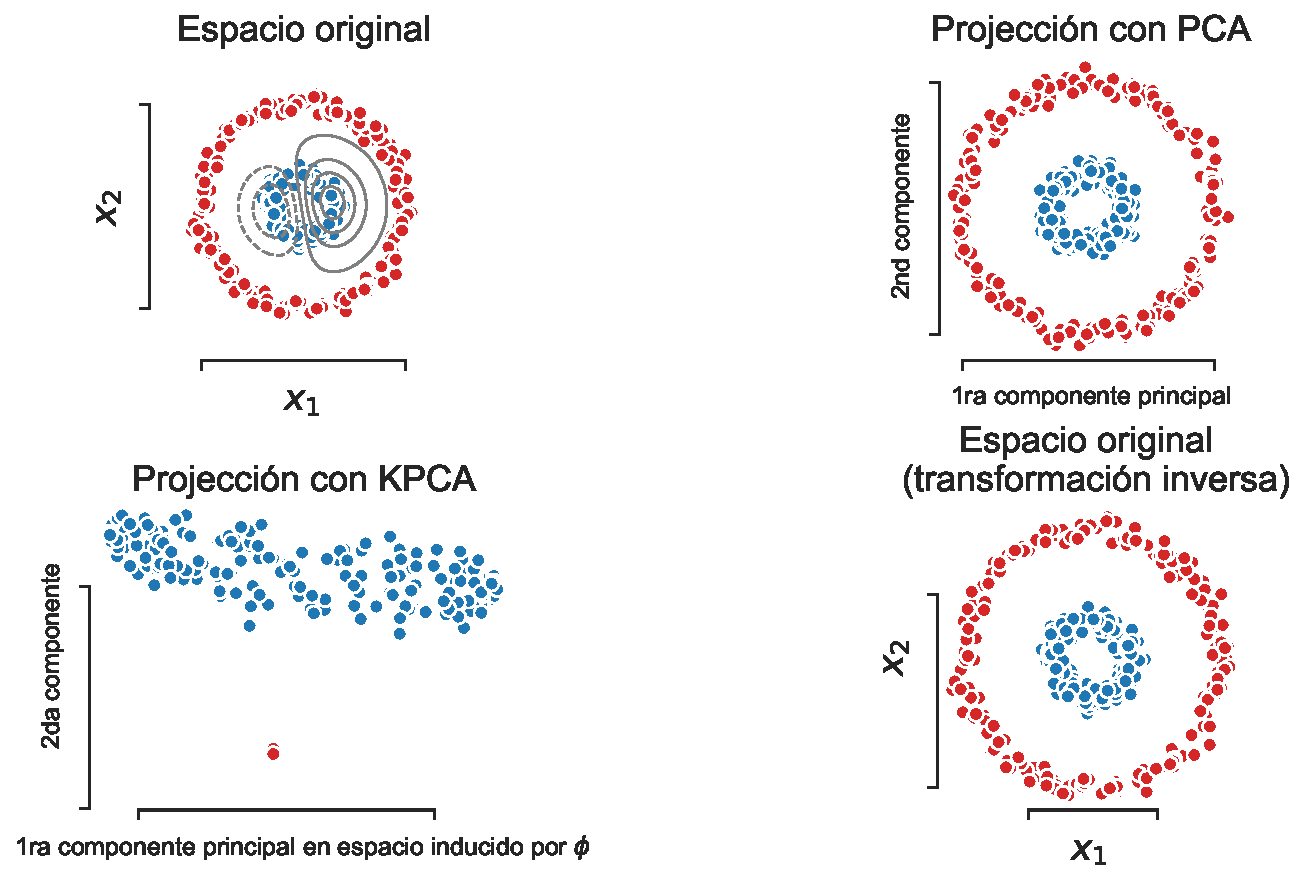
\includegraphics[width=0.6\linewidth]{../img/cap6_kpca.pdf}
    \caption{Ejemplo de KPCA sobre un conjunto de datos que no es linealmente separable.}
    \label{fig:kpca}
\end{figure}

\end{frame}

%Discriminante lineal de Fisher: idea general.
\begin{frame}{Discriminante lineal de Fisher: idea general}
	
Es posible interpretar el problema de clasificación como uno de \emph{reducción de dimensionalidad}: \pause

\begin{itemize}
	\item La reducción consiste representar nuestros datos  en solo una dimensión, la cual representa su grado de pertenencia a una clase. \pause
	\item Al proyectar un objeto $M$-dimensional en un espacio  1-dimensional, se pierde gran parte de la información, por lo que clases claramente separadas en el espacio $M$-dimensional puedan traslaparse al ser proyectadas a 1 dimensión.\pause
	\item Sin embargo, es posible ajustar el vector $a$ con la finalidad de obtener una proyección de $x$ que maximice el grado de separación entre clases.\pause
	\item Para el problema de clasificación binaria de $x\in \R^M$, se proyecta $x$ en un espacio \textbf{unidimensional} con respecto a un vector $a\in\R^M$ de acuerdo a:
\begin{equation*}
	y = a^\top x,
\end{equation*}
donde se puede definir un umbral $b$ para asignar $x$ a $\cC_1$ si $y+b\geq 0$ y $x$ a $\cC_2$ en caso contrario. Esto recupera el modelo lineal para clasificación.
\end{itemize}
	
\end{frame}

%Discriminante lineal de Fisher: primera formulación.
\begin{frame}{Discriminante lineal de Fisher: primera formulación}
Se buscará un vector $a$ con la finalidad de obtener una proyección de $x$ que maximice el grado de separación entre clases. Se propone el siguiente esquema:\pause

\begin{itemize}
	\item Cardinales de clase: $N_1 = |\{x\in\datos:x\in\cC_1\}|$ y $N_2 = |\{x\in\datos:x\in\cC_2\}|$.\pause
	\item Estos permiten calcular los promedios muestrales (centros de masa) de cada clase: 
\begin{equation*}
	\mu_1=\frac{1}{N_1}\sum_{n\in\mathcal{C}_1}x_n
	\quad\quad\quad
	\mu_2=\frac{1}{N_2}\sum_{n\in\mathcal{C}_2}x_n,
\end{equation*}
\pause
	\item De esta forma, la medida más simple de separación entre las proyecciones de las clases sobre $a$ es la distancia entre las medias  de sus proyecciones:
\begin{equation*}
	m_1 - m_2 = a^\top(\mu_1-\mu_2),
\end{equation*}
donde $m_k= a^\top\mu_k$ corresponde al promedio de los elementos de  la clase $\mathcal{C}_k$ proyectado sobre el  vector $a$ (centro de masa sobre la recta).
	\item el $a$  que maximiza la expresión anterior es simplemente $a\propto (\mu_1-\mu_2)$
\end{itemize}

\end{frame}


%Discriminante lineal de Fisher: primera formulación (desventaja).
\begin{frame}{Discriminante lineal de Fisher: primera formulación (desventaja)}

El problema de este enfoque es que pueden existir 2 clases bien separadas en el espacio $M$-dimensional, pero que al proyectar los datos sobre la recta que une sus promedios, las proyecciones de cada clase se traslapen. \pause

\begin{figure}[H]
	\centering
	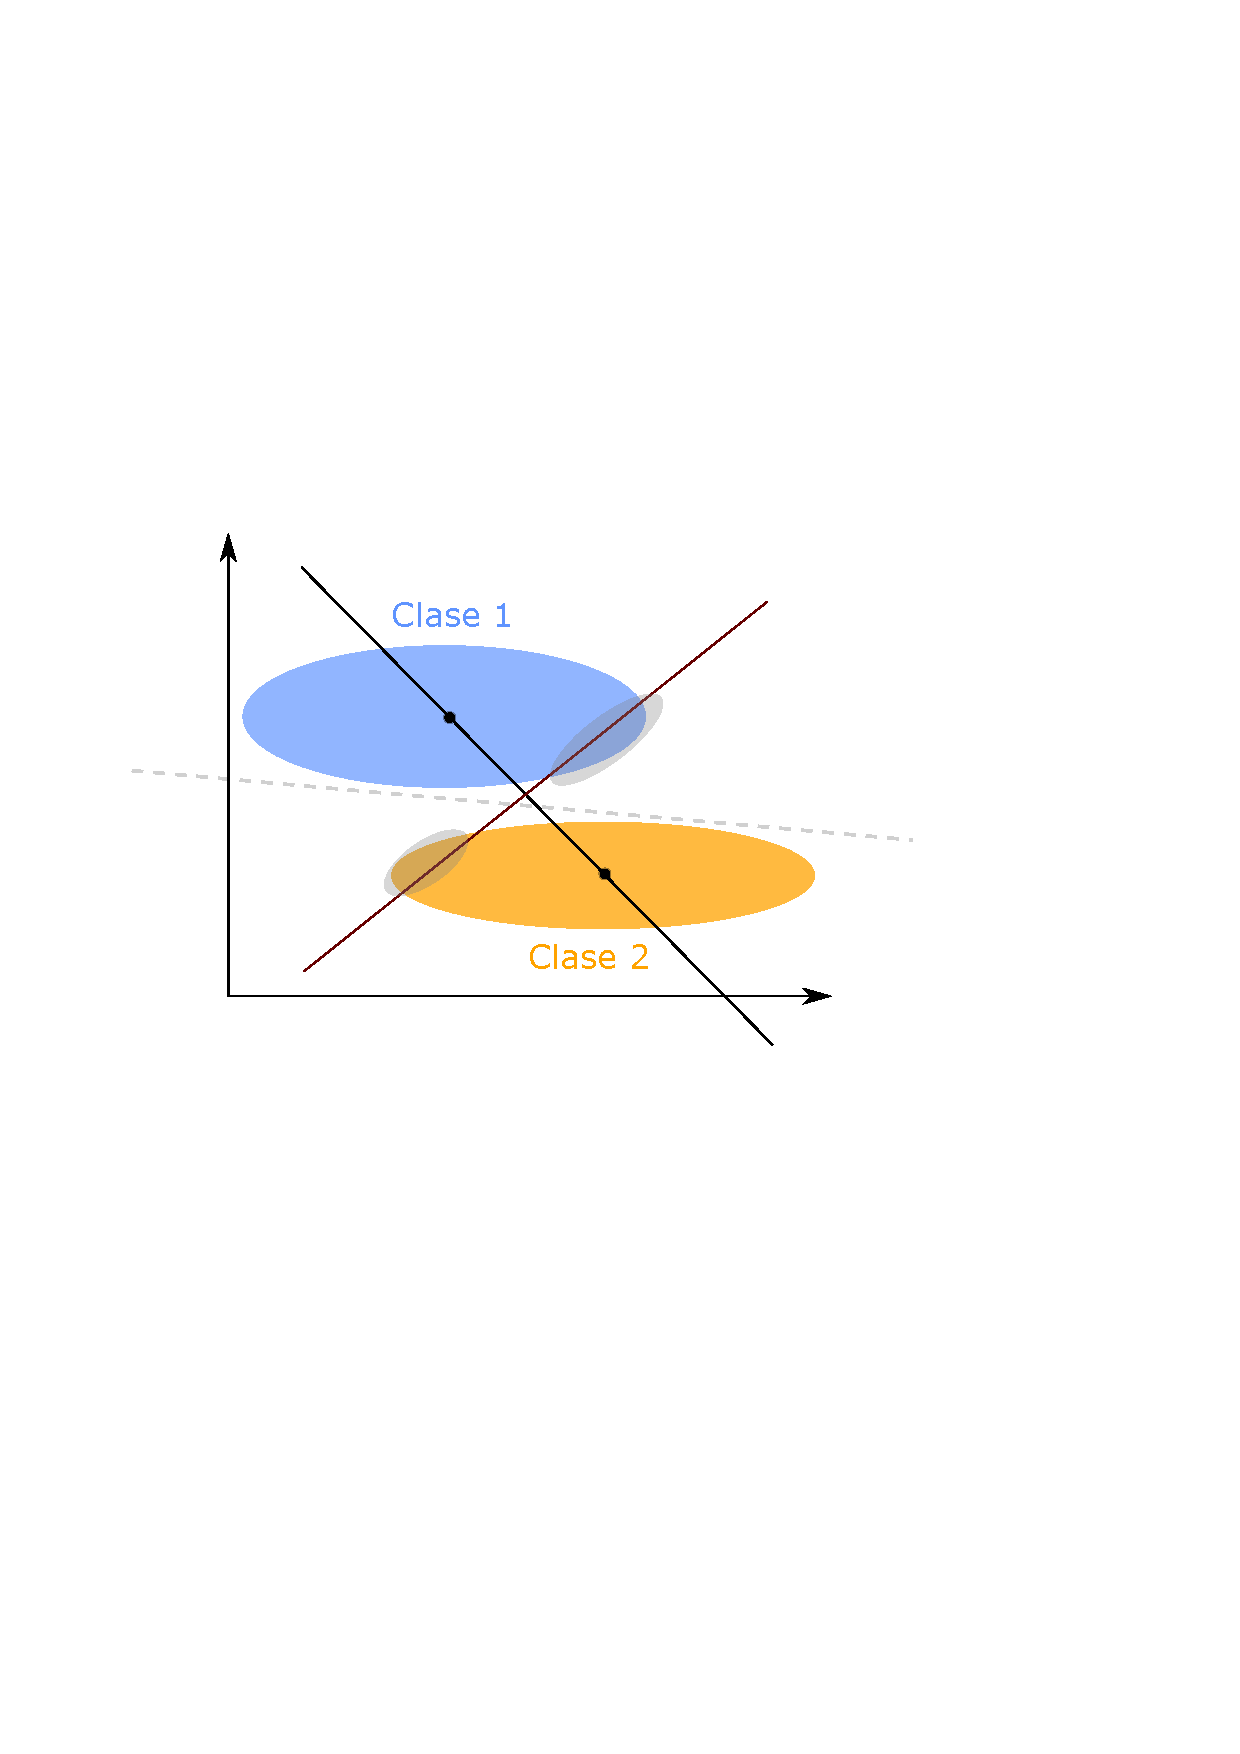
\includegraphics[width=0.6\textwidth]{../img/cap6_fisher.pdf}

\end{figure}

\end{frame}


%Discriminante lineal de Fisher: segunda formulación.
\begin{frame}{Discriminante lineal de Fisher: segunda formulación}

Para resolver este problema, Fisher propuso el siguiente esquema:

\begin{itemize}
	\item maximizar la distancia entre las medias de las clases proyectadas (primera formulación).\pause
	\item Adicionalmente, minimizar la dispersión de los elementos de una misma clase con el objetivo de disminuir el traslape entre las proyecciones de las clases.\pause
\end{itemize}

 Como medida de dispersión, se define la varianza muestral proyectada de los elementos de la clase $\cC_k$ mediante
\begin{align*}
	s_k^2 &= \sum_{n\in \mathcal{C}_k}(a^\top(x_n-\mu_k))^2= \sum_{n\in \mathcal{C}_k}(y_n-m_k)^2,
\end{align*}
donde el factor de correción $\frac{1}{N_k-1}$ fue omitido ya que de lo contrario, todas las clases pesarían lo mismo sin importar la cantidad de elementos de la clase.\\~\ \pause

Lo anterior permite definir la siguiente función objetivo:
\begin{equation*}
J(a) = \frac{(m_1-m_2)^2}{s_1^2+s_2 ^2}.
\end{equation*}

\end{frame}


%Discriminante lineal de Fisher: segunda formulación.
\begin{frame}{Discriminante lineal de Fisher: segunda formulación}

Se puede expresar este costo directamente como función del vector de proyección $a$:
\begin{equation*}
	J(a) = \frac{(m_1-m_2)^2}{s_1^2+s_2 ^2} = \frac{a^\top S_B a}{a^\top S_Wa},
\end{equation*}
donde la matriz de covarianza entre clases $S_B$ y matriz total de covarianza dentro de clases $S_W$ están dadas por
\begin{align*}
	S_B &= (\mu_1-\mu_2)(\mu_1-\mu_2)^\top\\
	S_W &= \sum_{n\in \cC_1}(x_n-\mu_1)(x_n-\mu_1)^\top +
	\sum_{n\in \cC_2}(x_n-\mu_2)(x_n-\mu_2)^\top. 
\end{align*}

\end{frame}


%Discriminante lineal de Fisher: optimización.
\begin{frame}{Discriminante lineal de Fisher: optimización}

Aplicando la condición de primer orden para $J(a)=\frac{a^\top S_B a}{a^\top S_Wa}$, obtenemos que el vector $a$ óptimo debe cumplir
\begin{equation*}
	(a^\top S_B a)S_W a = (a^\top S_W a)S_B a.	
\end{equation*}
\pause
\begin{itemize}
	\item La norma del vector  $a$ es irrelevante (solo interesa su orientación), con lo que  ignorando los escalares $a^\top S_B a$ y $a^\top S_W a$ tenemos que la relación de optimalidad es $S_W a \propto S_B a$.\pause
	\item por la definición de $S_B$, sabemos que $S_B a\propto(\mu_1-\mu_2)$, con lo que la relación de optimalidad se convierte en es $S_W a \propto (\mu_1-\mu_2)$.
\end{itemize}
\pause
Consecuentemente, el vector optimo $a$ en el  criterio de Fisher debe cumplir
\begin{equation*}
	a \propto S_W^{-1}(\mu_1-\mu_2).
\end{equation*}

\end{frame}

%Discriminante lineal de Fisher: ejemplo.
\begin{frame}{Discriminante lineal de Fisher: ejemplo}
En la siguiente figura se observa el  discriminador lineal que solo considera los promedios (izquierda) y la corrección de Fisher (derecha). 
\begin{figure}[H]
	\centering
	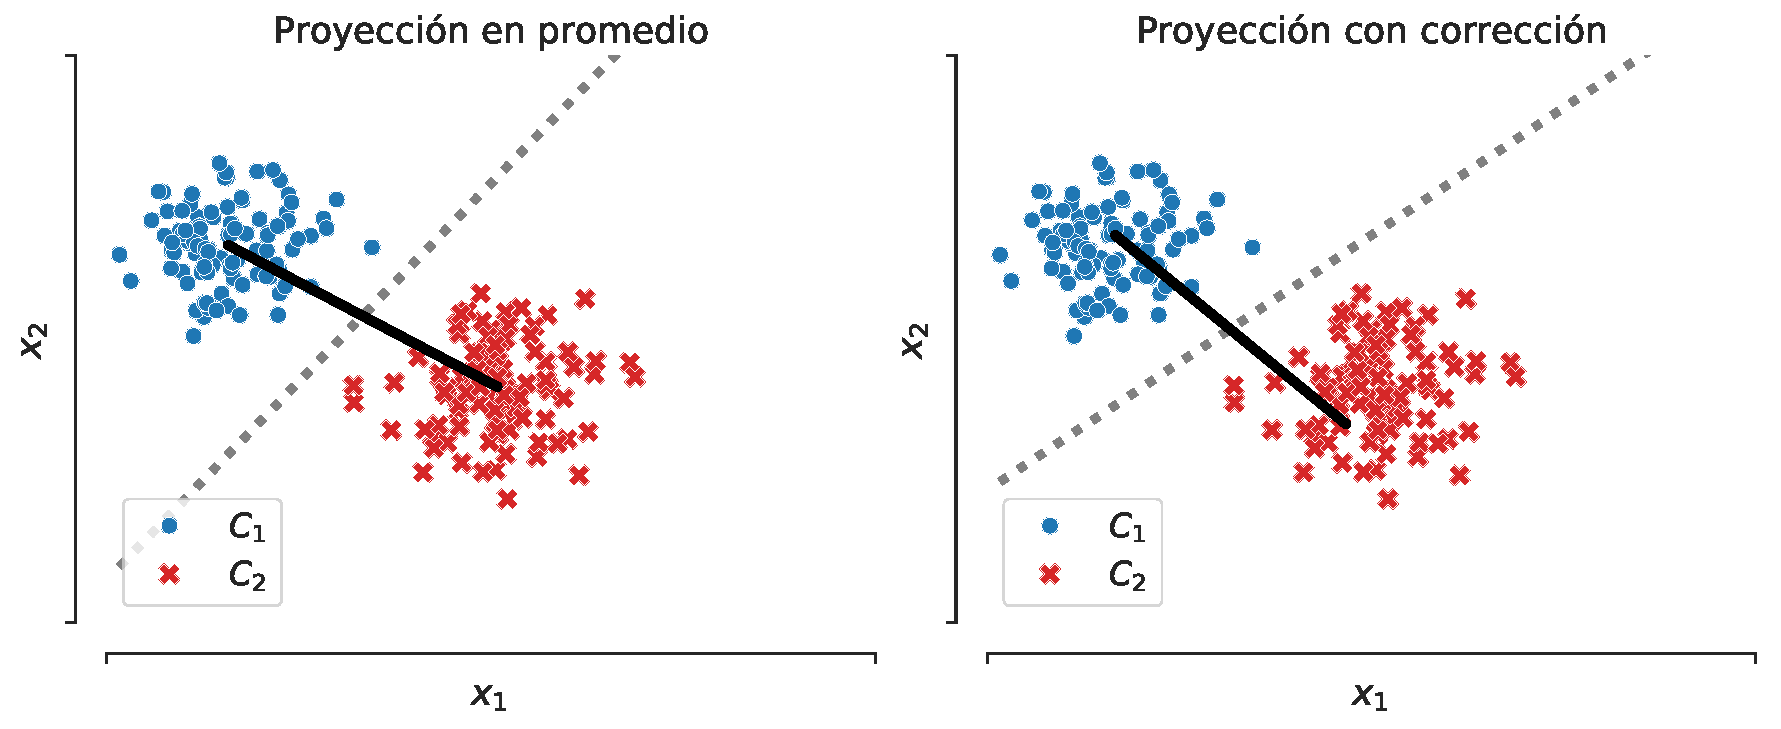
\includegraphics[width=0.8\textwidth]{../img/cap6_dos_clases_proyeccion.pdf}

\end{figure}
\end{frame}


\end{document}
